\documentclass[twocolumn]{IEEEtran}

\usepackage[utf8]{inputenc}
\usepackage{amssymb}
\usepackage{amsmath}
\usepackage{color}
\usepackage[english]{babel}
\usepackage{graphicx}
\usepackage{multicol}
\usepackage[labelsep=endash]{caption}
\usepackage[dvipsnames]{xcolor}

\renewcommand{\figurename}{Fig.}

\graphicspath{ {images/} }

\definecolor{pink}{rgb}{0.98, 0.52, 0.9}
\definecolor{gray}{rgb}{0.41, 0.41, 0.41}

\begin{document}

\title{Unums: \break A Number Format For Modern Computation}
\author{Emmanouil Raptakis}

\maketitle

\begin{abstract}
The standard number format for computing in today's world is the IEEE floating point format, however there exist many undesirable qualities surrounding this format. As a result the idea of the unum format was devised in 2014 by John Gustafson and in this text I describe the issues surrounding the floats such as incorrect results from computations, fixed lengths of floats and unnecessary power costs while also demonstrating how the unum representation resolves these issues and represents a numerical format for computation more in line with the 'parameters' of the modern world in order to extend communications on the issue.
\end{abstract}

\section{What is a Unum?}
The Unums, which I will also refer to as the set $\mathbb{U}$ are a set of representations of $\mathbb{R}$ (the set of real numbers) which build upon, and hence form a superset of the IEEE floating point numbers (the current standard in computation). In addition to forming a superset, the unums possess various useful properties systems which are not exhibited by the floats. Namely, these are:
\break
\centerline{$\forall a,b,c \in \mathbb{U}$}
\begin{enumerate}
	\item $(a + b) + c = a + (b + c)$ ; Associativity 
	\item $(a + b) \in \mathbb{U}$ ; Closure
	\item $\forall x \in \mathbb{R}$ $ \exists u \in \mathbb{U}$ where $u$ is the representation of $x$ in the current unum  	     	          environment, independent of the (maximum) number of bits allocated to the unum
\end{enumerate}
In addition it is useful to note that a key property of unums, which allows for the reduction of power costs, is their ability to dynamically adjust their precision / the number of allocated bits (which also is useful as it does not require the programmer to have to deal with allocating the correct type of float for a calculation). As an example, in the unum $\left\{3,4\right\}$ environment, which is characterised by a dynamic range similar to an IEEE single precision float and slightly more precision than a half precision float the number $1$ is represented as follows:

\begin{figure}[h]

\begin{center}

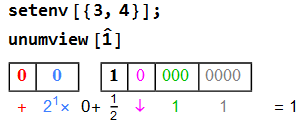
\includegraphics[scale=0.7]{unumview1}
\caption{$1$ in the unum format represented using the $\left\{3,4\right\}$ environment}

\end{center}

\end{figure}

As we see from Figure 1, far fewer bits are required to store $1$ as a unum than as a float of similar range and precision; the extra bits  allocated to floats would, in this situation only serve the purpose of providing an unnecessary number of zeros after the decimal point (why should a simple number such as $1$ require the exact same number of bits to describe it as $\pi$?) Hence, by adopting an alternative to the IEEE floats, we can reduce power costs associated with the transportation of these "dead weight bits" at the expense of performing additional computations to dynamically adjust our precision.

%Add additional information about the specifics of power costs associated with moving bits.
\subsection{What does a Unum look like?}
Unums expand on the IEEE float, adding 3 additional fields (which together compromise what is known as the \textbf{utag}) to the original 3 fields, as  we see in Figure 1:

\begin{enumerate}

% Read up more on exponent and fraction meaning

	\item \textcolor{red}{$\textbf{\Large{s}}$} - The sign bit reflects the sign of a number (\textcolor{red}{1} represents $u <    	0$ and \textcolor{red}{0} represents $u > 0$)
	\item \textcolor{blue}{$\textbf{\Large{e}}$} - The exponent field reflects the scale of the number that we wish to represent
	\item \textcolor{black}{$\textbf{\Large{f}}$} - The fraction field reflects the 'precision' of the number we are representing
	\item \textcolor{pink}{$\textbf{\Large{u}}$} - The ubit reflects if we are dealing with an exact float or an interval 	     between two exact floats
	\item \textcolor{Green}{$\textbf{\Large{es-1}}$} - The exponent size field is a number 1 less than the length of the exponent 	    field (reducing the size by 1 allows us to save a bit since $\Large{\textbf{\textcolor{blue}{esize}} \geq 1}$
	\item \textcolor{gray}{$\textbf{\Large{fs-1}}$} - The fraction size field is a number 1 less than the length of the fraction 	    field (reducing the size by 1 allows us to save a bit since $\Large{\textbf{\textcolor{black}{fsize}} \geq 1}$
\end{enumerate}
To convert an exact unum to a real number we then use the following equation to perform the conversion:
\begin{equation}
x = (-1)^{\textcolor{red}{\textbf{s}}}}\times
\[ \begin{cases}
	2^{\textcolor{blue}{\textbf{e}}-2^{\textcolor{Green}{\textbf{es-1}}}}\times \left( \cfrac{\textbf{f}}{2^{\textcolor{gray}{\textbf{fs}}}} \right) & $if the \textcolor{blue}{\textbf{e}} field is $0$$\\
	\infty & $\scriptsize{if all the bits in the \textcolor{blue}{\textbf{e}}, \textcolor{black}{\textbf{f}}, 
	\textcolor{Green}{\textbf{es-1}}, \textcolor{gray}{\textbf{fs-1}} fields are 1}$\\
	2^{\textcolor{blue}{\textbf{e}}-2^{\textcolor{Green}{\textbf{es-1}}}}\times \left( {1 + \cfrac{\textbf{f}}{2^{\textcolor{gray}{\textbf{fs}}}}\right) & $otherwise$\\
\end{cases}
\]
\end{equation}
To complete the unum format the purpose of the ubit need also be shown. If the \textbf{\textcolor{pink}{ubit}} $=0$, then we are simply dealing with an exact float and we use (1) to compute the float. When we are dealing with some number $|x| < \infty$ with the \textbf{\textcolor{pink}{ubit}} $ = 1$, then the unum represents an open interval between the exact float (as computed with (1)) and the neighbouring float which is further from 0. Since this definition does not make much mathematical sense for $|x| = \infty$ so we re-purpose these representations; a unum with $s=0$ and all other bits equal to $1$ represents the quiet NaN and the unum with all bits equal to $1$ represents the signalling NaN. When declaring a unum, since the number of bits is not a fixed quantity, we instead set a parameter requiring 2 arguments (the \textbf{\textcolor{RoyalPurple}{ess}} and \textbf{\textcolor{Orange}{fss}}}, the size of the \textbf{\textcolor{Green}{es-1}} and \textbf{\textcolor{gray}{fs-1}} fields respectively) which is known as the environment of the unum and is denoted as $\left\{\textbf{\textcolor{RoyalPurple}{ess}},\textbf{\textcolor{Orange}{fss}}\right\}$, an example of which exists in Figure 1. The required environment for some computation can be easily estimated by the programmer by thinking about the overall accuracy that is required for the task since the computer will be dynamically adjusting the unum towards an optimal representation as well as having the ability to dynamically adjust the environment for a specific calculation in order to return more accourate results (the returned result will still be in the original environment).

\subsection{How can Unums lower power costs?}
\textbf{IN PROGRESS} \break
The addition of a utag in a unum (particularly the \textbf{es-1} and \textbf{fs-1} fields) allows for variable bit lengths in their representation. This effectively results in being able to reduce the number of required bits (and in turn significantly reduce the costs associated with transportation of bits through the large DRAM wires that consume a lot of power) at the added 'tax' of additional logic operations being required. The reason for favouring this approach is that in our modern society the cost of logic / transistors is incredibly low. 
\section{Rounding Errors in the IEEE floats}
In the IEEE standard, the most commonly used method of rounding is known as Bankers Rounding (Rounding to the nearest even). In essence the method simply rounds floats to the nearest representable float and in the situation where the float is equidistant from the two nearest floats it rounds towards the nearest even number. The method is praised for being "unbiased", however the validity of the statement is questionable; the expectation value of the error from this method will tend to zero as the number of operations $n \rightarrow \infty$, however the issue that arises is that the variance of the error term will also increase in this process, giving a potentially significant deviation from the correct result (which can and has been previously disastrous). Two examples of this issue can be demonstrated through what I will refer to as "Short Triangles" and "The Patriot Issue". As an aside, the way that unums resolve the issue of rounding is that they simply \textbf{DO NOT ROUND}. Rather, if a result lies between two exact floating points, then the ubit "activates/becomes a $1$" and the result is recorded as an open interval between the two exact floats. Analogously we can think of the storing of $\pi$ as a float vs as a unum. With a relatively low number of bits we might be able to represent it as $3.141$ or $3.142$, both of which are incorrect since $\pi$ is infinitely precise, but we are only working with a finite number of bits / the result is rounded. Rather than using an infinite number of bits to express $\pi$ correctly or accepting the rounded result, the unum approach would instead use the ubound $\pi  = (3.141,3.142)$, which is a mathematically correct statement ($\pi$ does lie somewhere between the two specified floats!).

\subsection{Short Triangles}
As an example of the impact that rounding errors can have on numerical calculations can be illustrated using Herons Formula for the area of a very short triangle (short being defined as being of the order of ULPs\footnote{A ULP / Unit in the Last Place or Unit of Least Precision is the 'spacing' between floating points; a more in-depth review is present in Appendix A} of the type of floating point being used; in the example a double precision float is utilised, which has a ULP of $2^{-52}$)

\begin{theorem}
\textit{\textbf{Herons Formula}: For any Triangle of side lengths $a, b, c$ }
\break
$A = \sqrt{s(s-a)(s-b)(s-c)}$ where $s = \cfrac{a + b + c}{2}$
\break
\end{theorem}

As a specific example we can use $b = 7.0$ and \break
$a = c = {7.0 + 2^{-52}}$ as the sides of the Triangle and compute the area with Herons Formula when storing the variables as 64-bit floats v.s. 96-bit floats.

\begin{figure}[h]

\begin{center}

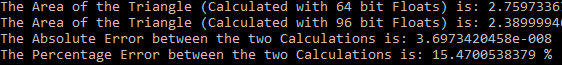
\includegraphics[scale=0.7]{Single_Triangle}
\caption{The result when comparing using double and triple precision floats for the Triangle calculation turns out to be significant!}

\end{center}

\end{figure}

\subsection{The Patriot Issue}
During the Gulf War the US utilised a missile defence systems known as the Patriots. They were tasked with the tracking and interception of Iraqi scud missiles. On the 25th of February 1991 at Dhahran in Saudi Arabia, the defence system failed to track an incoming enemy scud missile aimed at the nearby army barracks, leading to the deaths of 28 American soldiers and injuring about 100 others. The failure to track the missile resulted from an issue in the software when converting the time from an integer number of tenths of a second to its floating point representation (however in the floats 0.1 is nonterminating; it cannot be represented as a finite number of bits, so there will be an error due to rounding as the system will have to resort to rounding resulting in tracking errors that worsened with the length of time that the system was operational. In Dhahran the battery was continuously operational for a period of over 100 hours at the time of the incident, hence the inaccuracies became large enough to result in a miscalculation of the trajectory of a tracked scud, which the system "lost" as it was looking in the wrong region and hence dismissed the scud as an error (which then crashed into the barracks and resulted in the disaster). From the official documents on the failure from the US General Accounting Office it is stated that at 100 hours of operation time, the inaccuracy in time amounts to $0.3433s$, leading to a shift in the Range Gate (the predictor for where the scud is expected to be at the time of the transmission of the next pulse) of $687m$, however this information was unknown to the soldiers at the time, who were simply told to not leave the Patriot on for extended periods of time. The advantage of utilising the unum approach is then also easily understood from this scenario; with the ability of the unums to accurately quantify 'rounding errors' it is easier to make decisions as we have more information available. 

\begin{figure}[h]

\begin{center}

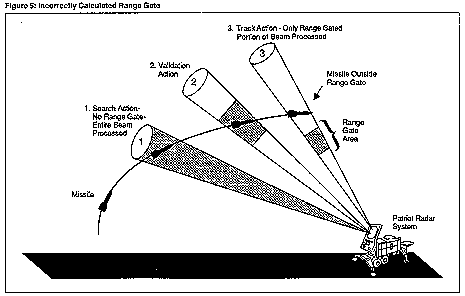
\includegraphics[scale=0.7]{missile}
\caption{The Official Depiction of the error in the tracking system of the Patriot, published by the US GAO}

\end{center}

\end{figure}


\end{document}